\chapter{Project Plan}

At this stage, it is important to try and plan ahead to create a realistic expectation of what may completed in the time allocated for this project. I have identified several tasks and milestones to consider for this project, and produced an approximation of how long each of these will take in relation to the project schedule. \\

Some milestones worth mentioning are:

\begin{enumerate}
	\item \textbf{Exams week} - As expected during this time and leading up to it, development and project work will be heavily reduced. This also marks the milestone whereafter I can work on this project full time. Up until this deadline, my time will have been split with other university modules and studying, therefore estimated feature development time is inflated to reflect this.
	\item \textbf{Project Audit} - It is important to stop and reflect during project development to assess progress done. I have assigned a project audit around halfway through the technical development timeline to assess the architecture of the code base, as well as its usability and visual appeal. These features are important to assess and maintain up to date to create a useful tool, and if left unmanaged for the entirity of development will heavily degrade the quality of the final project. I assign some time thereafter to make amends to the project as a result of this.
	\item \textbf{Extension} - I assign some time to be able to write an XML attack analysis module. If written, this would be a hard extension to add to the tool, as XML attacks have several input vectors, and present a difficult challenge to exploit. The time allocated to this may also serve as a potential soak up of delays in the project, should they happen, so also acts as a safeguard.
\end{enumerate}

The next pages include Gantt charts with approximations of how work will be spread out throughout the project. \emph{\textbf{N.B} - the time period observed in these graphs overlaps}.

\newpage

\begin{figure}[h]
	\centering
	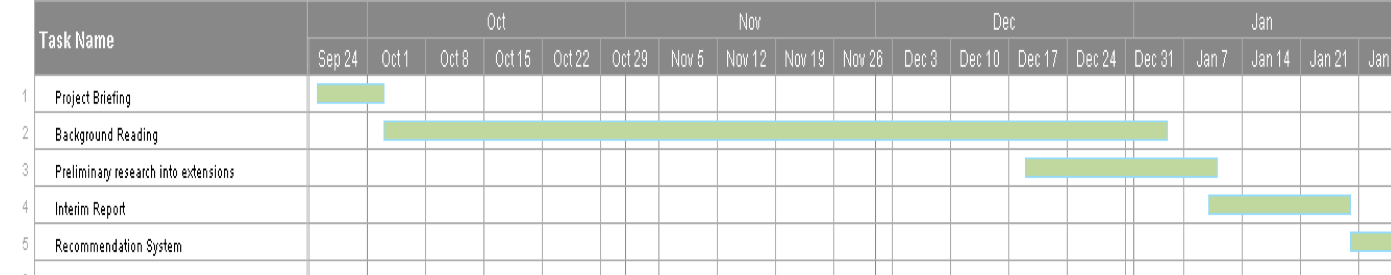
\includegraphics[angle=90]{images/plan6.png}
	\label{fig:test}
\end{figure}

\begin{figure}[h]
	\centering
	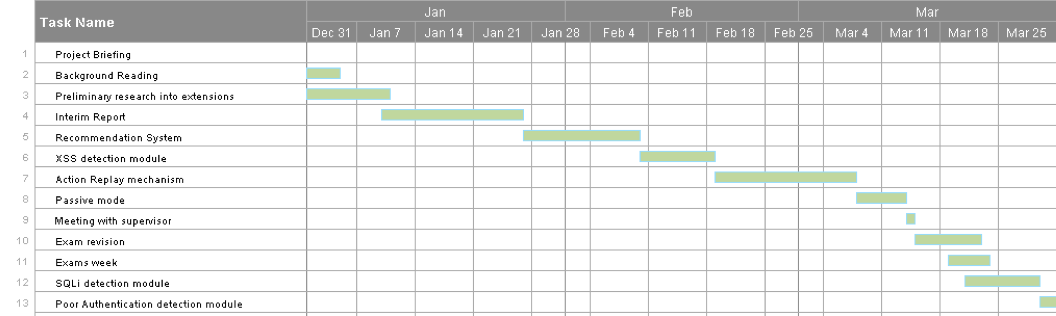
\includegraphics[angle=90]{images/plan4.png}
	\label{fig:test}
\end{figure}
\newpage

\begin{figure}[h]
	\centering
	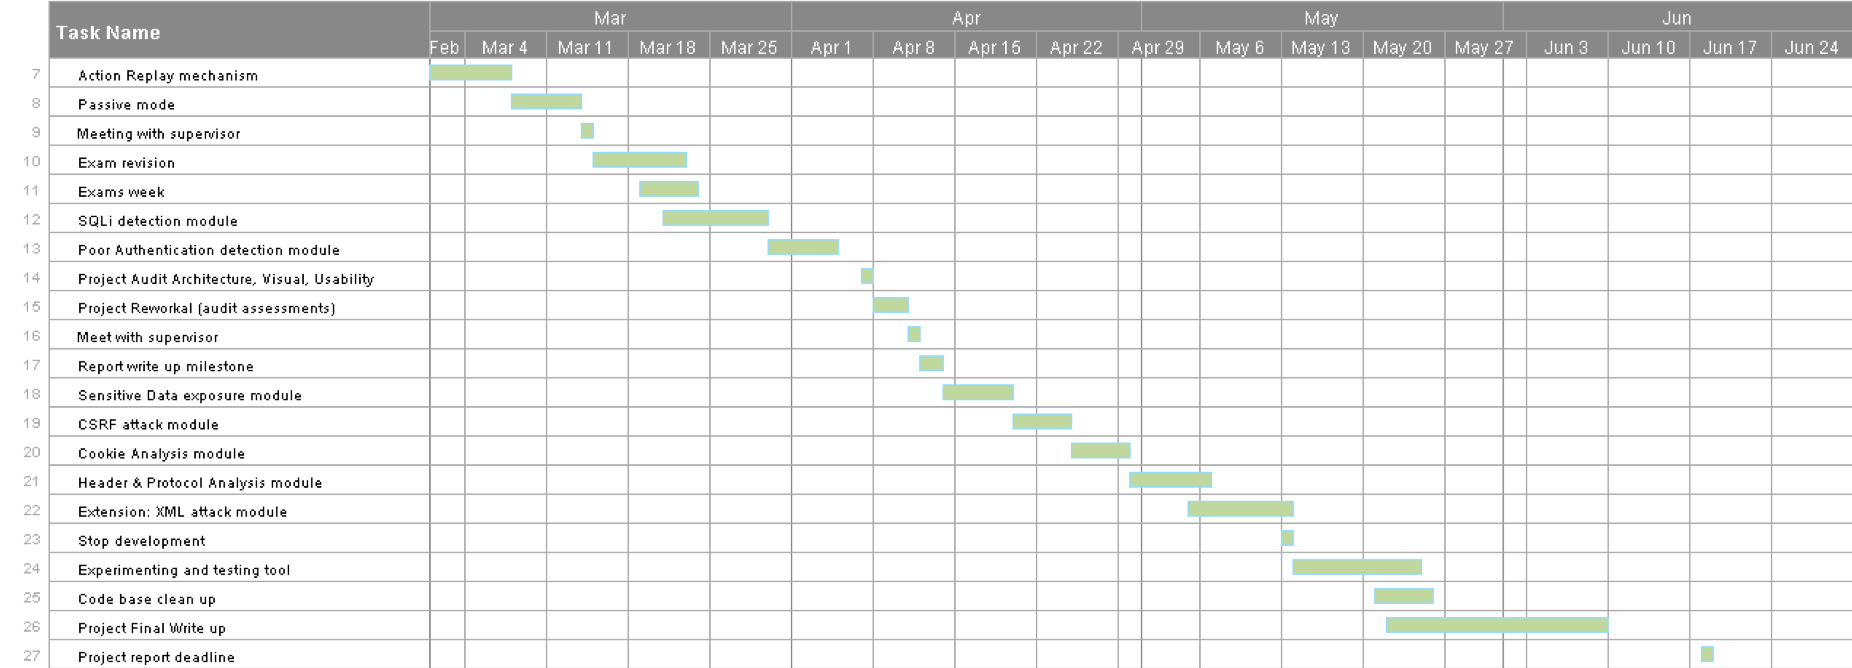
\includegraphics[width=\textheight, angle=90]{images/plan2.png}
	\label{fig:test}
\end{figure}


